\documentclass[usenames,dvipsnames,8pt,aspectratio=169]{beamer}
\usepackage{amsmath,amsfonts,amssymb}
\usepackage{mathtools}
\usepackage{etex} %for Windows
\usepackage[utf8]{inputenc}
\usepackage[english, russian]{babel} 
%\usepackage{microtype}			% Better interword spacing and additional kerning.
\usepackage{ellipsis}			% Adjusted space with \dots between two words.
\usepackage{graphicx}
\usepackage{pstricks}

\usepackage{xcolor}


\usepackage{changepage}

\usepackage{algorithm}
\usepackage{algpseudocode}
%\usepackage[]{algorithm2e}
%\usepackage{algorithmic}

%\usepackage{tcolorbox}

\usepackage{tikz}
\usetikzlibrary{tikzmark,calc}
\usetikzlibrary{positioning, backgrounds}
\usetikzlibrary{arrows, chains, matrix, scopes, patterns, shapes, fit}
\usetikzlibrary{mindmap,trees,shadows}
\usetikzlibrary{decorations.pathreplacing}
\usetikzlibrary{crypto.symbols}

\usepackage{pgfplots}


\usepackage{listings} % for C++ code

\usepackage{braket}
%\usepackage[braket, qm]{qcircuit}



\usepackage[T1]{fontenc}
%\usepackage[sfdefault,scaled=.85]{FiraSans}
%\usepackage{newtxsf}
%\usepackage[nomap]{FiraMono}





\usefonttheme[onlymath]{serif}
\renewcommand\sfdefault{cmbr}

\renewcommand{\bfdefault}{sb}

\definecolor{CharCoalDark}{RGB}{13, 16, 19}
\definecolor{Orange}{RGB}{255, 165,0}
\definecolor{DarkOrange}{RGB}{255, 165,0}
\definecolor{LightSalmon}{RGB}{255, 160, 122}
\definecolor{LeafGreen}{RGB}{34, 139,  34}
\definecolor{Coral}{RGB}{255, 127, 80}
\definecolor{DarkTurquoise}{RGB}{0, 206, 209}

%\newtheorem{defRus}{Определение}
%\newtheorem{thmRus}{Теорема}
%s\newtheorem{corRus}{Следствие}


\setbeamercolor{background canvas}{bg=CharCoalDark}

\setbeamerfont{title}{series=\bfseries}
\setbeamercolor{title}{fg=Orange}
\setbeamercolor{section in toc}{fg=white}
\setbeamercolor{frametitle}{fg=Orange}
\setbeamercolor{normal text}{fg=white}
%\setbeamercolor{normal text}{fontsize=12pt}
\setbeamercolor{itemize item}{fg=Orange}
\setbeamercolor{enumerate item}{fg=Orange}
\setbeamercolor{enumerate item item}{fg=Orange}
\setbeamercolor{itemize item item}{fg=Orange}
\setbeamercolor{enumerate item}{fg=Orange}
\setbeamercolor{block title}{bg=DarkOrange,fg=white}
\setbeamerfont{block title}{series=\bfseries}

\setbeamertemplate{itemize item}[circle]
\setbeamertemplate{eumerate subitem}{\color{Orange}[$\checkmark$]}
\setbeamertemplate{itemize subitem}{\color{Orange}\Large$\textbullet$}
\setbeamertemplate{itemize subitem}{\color{Orange} \tiny $\blacksquare$}

% footnote without a marker
\newcommand\blfootnote[1]{%
	\begingroup
	\renewcommand\footnoterule{}
	\renewcommand\thefootnote{}\footnote{#1}%
	\addtocounter{footnote}{-1}%
	\endgroup
}

\newcommand*{\Scale}[2][4]{\scalebox{#1}{\ensuremath{#2}}}%

\newcommand\Item[1][]{%
	\ifx\relax#1\relax  \item \else \item[#1] \fi
	\abovedisplayskip=0pt\abovedisplayshortskip=0pt~\vspace*{-\baselineskip}}

%\pgfdeclareradialshading{ring}{\pgfpoint{0cm}{0cm}}%
%{rgb(0cm)=(1,1,1);
%	rgb(0.7cm)=(1,1,1);
%	rgb(0.719cm)=(1,1,1);
%	rgb(0.72cm)=(0.975,0,0);
%	rgb(0.9cm)=(1,1,1)}
%
%\usepackage[absolute,overlay]{textpos} %to clip to a corner
%\newcommand\FrameText[1]{%
%	\begin{textblock*}{\paperwidth}(\textwidth-35pt, 10 pt)
%		\raggedright #1\hspace{.5em}
%\end{textblock*}}

%\makeatletter
%\let\save@measuring@true\measuring@true
%\def\measuring@true{%
%	\save@measuring@true
%	\def\beamer@sortzero##1{\beamer@ifnextcharospec{\beamer@sortzeroread{##1}}{}}%
%	\def\beamer@sortzeroread##1<##2>{}%
%	\def\beamer@finalnospec{}%
%}
%\makeatother


\title{Лекция №2 \\[10pt]
	Часть 1. Блочный шифр.}

\date{ Елена Киршанова \\  \textbf{Курс ``Основы криптографии''} \\  }


\setbeamertemplate{navigation symbols}{} %removes navigation

% proper highlightling of a code-snippet
\lstset{language=C++,
	keywordstyle=\color{magenta},
	stringstyle=\color{Goldenrod},
	commentstyle=\color{gray},
	breaklines=false,
	%morecomment=[l][\color{magenta}]{\#}
}

%\setlength{\parskip}{8pt}
% ==================================================================
% Definitions for this paper
% ==================================================================
\mathchardef\hyphen="2D

\usepackage{multirow}
\usepackage{multicol} % For multiple coloumn environments
%\usepackage{stmaryrd} % For set brackets
% \setlength{\columnsep}{15pt} % Defining the coloumn seperation
% \setlength{\columnseprule}{1pt} % Place a line between coloumns
% \newcommand{\tab}{\hspace*{2em}}

%subscripts

\newcommand*\SmallTextScript[2]{{\mathchoice{\displaystyle #2}
		{\textstyle #2}%dito
		{\scalebox{#1}{\ensuremath{\scriptstyle #2}}}%
		{\scalebox{#1}{\ensuremath{\scriptscriptstyle #2}}}%
}}


% ADVERSARIES AND SUCH
\newcommand*{\poly}{\ensuremath{\mathrm{poly}}}
\newcommand*{\eps}{\ensuremath{\varepsilon}}
\newcommand*{\alg}{\ensuremath{\mathcal{A}}}

% GROUPS/DISTRIBUTIONS/SETS/LISTS
\newcommand{\N}{{{\mathbb N}}}
\newcommand{\Z}{{{\mathbb Z}}}
\newcommand*{\IZ}{\ensuremath{\mathbb{Z}}}
\newcommand*{\IN}{\ensuremath{\mathbb{N}}}
\newcommand*{\IQ}{\ensuremath{\mathbb{Q}}}
\newcommand{\R}{{{\mathbb R}}}
\newcommand*{\IR}{{{\mathbb R}}}
\newcommand{\Zp}{\ints_p} % Integers modulo p
\newcommand{\Zq}{\ints_q} % Integers modulo q
\newcommand{\Zn}{\ints_N} % Integers modulo N
\newcommand{\F}{\ensuremath{\mathbb{F}}}
\newcommand{\CC}{\ensuremath{\mathbb{C}}}

\newcommand{\GF}{\ensuremath{\mathbb{F}_2}}
\newcommand{\GFn}{\ensuremath{\mathbb{F}^n_2}}

%%% ALGORITHMS/PROCEDURES %%%
\newcommand{\Dec}{\textsf{Dec}}
\newcommand{\Enc}{\textsf{Enc}}
\newcommand{\KeyGen}{\textsf{KeyGen}}
\newcommand{\Gen}{\textsf{Gen}}
\newcommand{\sk}{\textsf{sk}}
\newcommand{\pk}{\textsf{pk}}
\newcommand{\vk}{\textsf{vk}}
\newcommand{\mesS}{\ensuremath{\mathcal{M}}}
\newcommand{\keyS}{\ensuremath{\mathcal{K}}}
\newcommand{\cipS}{\ensuremath{\mathcal{C}}}
\newcommand{\tagS}{\ensuremath{\mathcal{T}}}
\newcommand{\mactag}{\textsf{tag}}
\newcommand{\Hash}{\ensuremath{\mathcal{H}}}
\newcommand{\EID}{\ensuremath{\mathtt{EphID}}}


\newcommand{\adv}{\ensuremath{\mathcal{A}}}

\newcommand{\LWE}{\mathsf{LWE}}
\newcommand{\DCP}{\mathsf{DCP}}
\newcommand{\EDCP}{\mathsf{EDCP}}
\newcommand{\UEDCP}{\mathsf{U \text{-} EDCP}}
\newcommand{\GEDCP}{\mathsf{G \text{-} EDCP}}



%% Landau and proba
\newcommand{\bigO}{\mathcal{O}}
\newcommand*{\OLandau}{\bigO}
\newcommand*{\WLandau}{\Omega}
\newcommand*{\xOLandau}{\widetilde{\OLandau}}
\newcommand*{\xWLandau}{\widetilde{\WLandau}}
\newcommand*{\TLandau}{\Theta}
\newcommand*{\xTLandau}{\widetilde{\TLandau}}
\newcommand{\smallo}{o} %technically, an omicron
\newcommand{\wLandau}{\omega}
\newcommand{\negl}{\mathrm{negl}}
\newcommand*\PROB\Pr 
\DeclareMathOperator*{\EXPECT}{\mathbb{E}}
\DeclareMathOperator*{\VARIANCE}{\mathbb{V}}
\DeclareMathOperator*{\LOGBIAS}{\mathbb{LB}}

\newcommand{\supp}{\ensuremath{\mathsf{sup}}}
\newcommand{\Distr}{\ensuremath{\mathcal{D}}}

% Lattices

% \newcommand{\coset}{\Lambda} % Lambda Lattice
% \newcommand{\cosetPerp}{\Lambda^{\bot}} % Lambda_Perp Lattice
% \newcommand{\gadget}{\textbf{G}} %Gaget matrix
% \newcommand{\mes}{\textbf{m}} %message vector
% \newcommand{\AMat}{\textbf{A}} %A matrices
% \newcommand{\BMat}{\textbf{B}} %B matrices
% \newcommand{\RMat}{\textbf{R}} %R matrices
% \newcommand{\HMat}{\textbf{H}} %H matrices
% \newcommand{\XMat}{\textbf{X}} %H matrices
% \newcommand{\mbar}{\bar{m}} %mBar dimension
% % \newcommand{\gauss}{\mathcal{D}} % gaussian distribution
% \newcommand{\Id}{\textbf{I}} % Identity matrix
% \newcommand{\er}{\textbf{e}} % gaussian distr. vectors
% % \newcommand{\cipher}{\textit{c}} % ciphertext
% \newcommand{\Olwe}{\mathcal{O}_{\textsf{LWE}}} %LWE oracle
% \newcommand{\OSample}{\mathcal{O}_{Sample}} %LWE oracle
% \newcommand{\SigmaB}{\boldsymbol{\Sigma}} %semi-deifinite matrix Sigma%
% % \newcommand{\mods}{\text{ mod}}


%Vectors and Matrices

\newcommand{\AMat}{\mathbf{A}} %A matrices
\newcommand{\BMat}{\mathbf{B}} %B matrices
\newcommand{\DMat}{\mathbf{D}} %Diagonal


\newcommand{\HMat}{\ensuremath{\mathbf{H}}}
\newcommand{\QMat}{\ensuremath{\mathbf{Q}}}
\newcommand{\Id}{\ensuremath{\mathbf{I}}}
\newcommand{\ZeroM}{\textbf{0}} % Zero matrix

\newcommand{\avec}{\ensuremath{\mathbf{a}}}
\newcommand{\bvec}{\ensuremath{\mathbf{b}}}
\newcommand{\cvec}{\ensuremath{\mathbf{c}}}
\newcommand{\evec}{\ensuremath{\mathbf{e}}}
\newcommand{\rvec}{\ensuremath{\mathbf{r}}}
\newcommand{\svec}{\ensuremath{\mathbf{s}}}
\newcommand{\tvec}{\ensuremath{\mathbf{t}}}
\newcommand{\vvec}{\ensuremath{\mathbf{v}}}
\newcommand{\zvec}{\ensuremath{\mathbf{z}}}
\newcommand{\xvec}{\ensuremath{\mathbf{x}}}
\newcommand{\yvec}{\ensuremath{\mathbf{y}}}
\newcommand{\uvec}{\ensuremath{\mathbf{u}}}
\newcommand{\zerovec}{\ensuremath{\mathbf{0}}}

\newcommand{\nth}{^{\mathrm{th}}}
\newcommand{\nd}{^{\mathrm{nd}}}

\newcommand{\RepMMT}{\ensuremath{\mathcal{R}_{\protect\SmallTextScript{0.70}{\texttt{MMT}}}}}
\newcommand{\RepBJMM}{\ensuremath{\mathcal{R}_{\protect\SmallTextScript{0.70}{\texttt{BJMM}}}}}
\newcommand{\XOR}{\ensuremath{\mathtt{3XOR}}}


% % % % % \newcommand{\mb}[1]{\mathbf{#1}} % does not compile otherwise
%%% Removed by Gotti; this is just asking to screw up with packages that (properly) define \mb (mathbold)

% \newcommand{\bL}{\|\bvec_1\|} % b1 length that appears way too often
% \newcommand{\dL}{\|\dvec_1\|} % b1 length that appears way too oftend

%Norms and Scalar products

\newcommand*\abs[1]{\left\lvert#1\right\rvert}
\newcommand*\norm[1]{\left\lVert#1\right\rVert}
\newcommand*\normalabs[1]{\lvert#1\rvert} 
\newcommand*\normalnorm[1]{\lVert#1\rVert}
\newcommand*\bignorm[1]{\bigl\lVert#1\bigr\rVert}
\newcommand*\bigabs[1]{\bigl\lvert#1\bigr\rvert}
\newcommand*\Bigabs[1]{\Bigl\lvert#1\Bigr\rvert}
\newcommand*{\ScProd}[2]{\ensuremath{\langle#1\mathbin{,}#2\rangle}} %Scalar Product
% \newcommand*{\ScProd}[2]{\ensuremath{\langle#1 \:{,}\:#2\rangle}} %Scalar Product
\newcommand*{\bigScProd}[2]{\ensuremath{\bigl\langle#1\mathbin{,}#2\bigr\rangle}} %Scalar Product
\newcommand*{\BigScProd}[2]{\ensuremath{\Bigl\langle#1\mathbin{,}#2\Bigr\rangle}} %Scalar Product
\newcommand{\dist}{\ensuremath{\text{dist}}}


%Some other math operators

\DeclareMathOperator{\Span}{Span} %span of vectors
\DeclareMathOperator{\vol}{\mathrm{vol}} %volume
\DeclareMathOperator{\LW}{LambertW} %Lambert W function
\DeclareMathOperator{\SD}{SD}
\DeclareMathOperator{\gradient}{grad}
\DeclareMathOperator{\TRACE}{Tr}
\newcommand*{\dDR}{\mathrm{d}} %de-Rham-Differential (the d in dx, dy, dz and so on)


%Lists
\renewcommand{\L}{\ensuremath{\mathcal{L}}}

\renewcommand{\P}{\ensuremath{\mathcal{P}}}

\newcommand*{\Lout}{\ensuremath{\L_{\mkern-0.5mu\protect\SmallTextScript{0.85}{\textup{out}}}}}
\newcommand*{\Sout}{\ensuremath{S_{\mkern-0.5mu\protect\SmallTextScript{0.85}{\textup{out}}}}}
\newcommand{\wt}{\ensuremath{\mathit{wt}}}


\newcommand*{\softO}{\widetilde{\bigO}}

\newcommand{\const}{\mathsf{c}} 


\newcommand{\transpose}{\mkern0.7mu^{\mathsf{ t}}}

%proper overline reduced by 1.5mu
\newcommand{\overbar}[1]{\mkern 1.5mu\overline{\mkern-1.5mu#1\mkern-1.5mu}\mkern 1.5mu}

\DeclareMathOperator{\erf}{erf} %error function
\DeclareMathOperator{\erfc}{erfc} %complementary error function
\newcommand{\Er}{\ensuremath{\mathrm{Er}}} %complementary error function


% LATTICES

\newcommand{\Lat}{\ensuremath{\mathcal{L}}}
\newcommand*{\Sphere}[1]{\ensuremath{\mathsf{S}^{#1}}}
%\DeclareMathOperator{\Conf}{Conf}
\newcommand{\Conf}{\mathcal{C}}

%Thick line for table
\setlength{\doublerulesep}{0pt}
\newcommand{\thickline}{\hline\hline\hline}


%circled text
\newcommand*\circled[1]{\tikz[baseline=(char.base)]{
    \node[shape=circle,draw,inner sep=0.3 pt] (char) {\scriptsize #1};}}


%Fix Algorithmicx package
\def\NoNumber#1{{\def\alglinenumber##1{}\State #1}\addtocounter{ALG@line}{-1}}

%For comments
\newcommand{\GColor}{ForestGreen}  %Damiens' color
\newcommand{\EColor}{MidnightBlue} %Elena's color

\newcommand*{\E}[1]{{\color{\EColor} #1} } 
\newcommand*{\G}[1]{{\color{\GColor} #1} } 

%Proper limit with the subscript underneath
% \newcommand{\Lim}[1]{\raisebox{0.5ex}{\scalebox{0.8}{$\displaystyle \lim_{#1}\;$}}}


%TIKZ dense dotted pattern

\pgfdeclarepatternformonly{my dots}{\pgfqpoint{-1pt}{-1pt}}{\pgfqpoint{2.0pt}{2.0pt}}{\pgfqpoint{2pt}{2pt}}%
{
	\pgfpathcircle{\pgfqpoint{0pt}{0pt}}{.35pt}
	\pgfpathcircle{\pgfqpoint{1pt}{1pt}}{.35pt}
	\pgfusepath{fill}
}


\tikzset{
	master/.style={
		execute at end picture={
			\coordinate (lower right) at (current bounding box.south east);
			\coordinate (upper left) at (current bounding box.north west);
		}
	},
	slave/.style={
		execute at end picture={
			\pgfresetboundingbox
			\path  (lower right)rectangle (upper left) ;
		}
	}
} %all defs
\begin{document}
	
\begin{frame}
	\titlepage
\end{frame}

%\begin{frame}{Админ}
%	
%	\Large
%	{\color{Orange} I. Симметрическая криптография} \\[10pt]
%	\begin{itemize}
%		\item 11/10 Псевдослучайные генераторы
%		\item 18/10 Блок-шифры
%		\item 25/10 Хэш-функции. Коды аутентификации сообщений 
%	\end{itemize}
%	
%	\vspace{20pt}
%	{\color{Orange} II. Асимметрическая криптография}
%	
%	\begin{itemize}
%		\item 1/11 Обмен ключами
%		\item 8/11 Цифровые подписи
%	\end{itemize}
%
%	\begin{itemize}
%		\item {\color{Orange}12/11 в  15:30-- 17:00 (?) } Зачет
%	\end{itemize}
%
%	
%\end{frame}


\begin{frame}{Блок-шифры: мотивация}
\LARGE 
	Симметричные шифр-схемы могут быть основаны на
	
	\begin{enumerate}
		\itemsep 10pt
		\item Потоковом шифре 
		\item Блочном  шифре
	\end{enumerate}

	\vspace{20pt}
	Блочные шифры лежат в основе {\color{Orange} шифрования с аутентификацией.}
\end{frame}


\begin{frame}{Блок-шифр: определение}
\LARGE

		{\color{Orange}\textbf{Блок-шифр}} -- это {\color{Orange} детерминированный} шифр $(\KeyGen, \Enc, \Dec)$ с  $\keyS, \mathcal{X}:=\mesS = \cipS, $ и эффективной функцией
		\[
			\Enc = f(k, \cdot): \mathcal{X} \rightarrow \mathcal{X}.
		\]
		
При этом выполняется
\begin{itemize}
	\item корректность $\implies f(k, \cdot)$ -- биекция для всех $k \in \keyS$ \\
	\item $|\mathcal{X}| < \infty$. \\
\end{itemize}

\vspace{20pt}

То есть, $f(k, \cdot)$ -- перестановка на $\mathcal{X}$. \\[10pt]


\end{frame}

\begin{frame}{Шифрование блока}
	\begin{tikzpicture}
	%\draw[-stealth, thick] (-1.8,-1.0) -- (-1.0,-1.0) node[above,midway]{\Huge $b$};
	\draw[fill=CharCoalDark, draw=white, opacity=0.5] (-1.0,0.0) rectangle (2.0,1.0)  node[color=white, opacity=1,align=center, pos=0.5]{
		\LARGE  {Откр. текст}  
	} node[above, midway, yshift=17pt]{\Large $n$ бит};
	\draw[-stealth, thick] (2.0,0.5) -- (3.0,0.5);

	\draw[fill=CharCoalDark, draw=white, opacity=0.5] (3.0,0.0) rectangle (5.0,1.0)  node[color=white, opacity=1,align=center, pos=0.5]{
		\LARGE  {$f$}  
	};
	\draw[-stealth, thick] (5.0,0.5) -- (6.0,0.5);
	
	\draw[fill=CharCoalDark, draw=white, opacity=0.5] (2.5,2.2) rectangle (5.5,3.0)  node[color=white, opacity=1,align=center, pos=0.5]{
		\LARGE  {Ключ}  
	} node[above, midway, yshift=12pt]{\Large $k$ бит};

	\draw[-stealth, thick] (4.0,2.2) -- (4.0,1.0);
	
	\draw[fill=CharCoalDark, draw=white, opacity=0.5] (6.0,0.0) rectangle (9.0,1.0)  node[color=white, opacity=1,align=center, pos=0.5]{
		\LARGE  {Шифр-текст}  
	} node[above, midway, yshift=17pt]{\Large $n$ бит};
	\end{tikzpicture}
	
	\vspace{20pt}
	\LARGE
	Примеры:\\
	\begin{itemize}
		\item AES: $n = 128$, $k = 128, 192, 256$
		\item ГОСТ 34.12-2018: $n=128$, $k=256$ (Кузнечик)
	\end{itemize}
\end{frame}

\begin{frame}{Безопасность блочного шифра $\Pi = (\KeyGen, \Enc = f, \Dec = f^{-1})$}
\Large
 
		$f(k, \cdot): \mathcal{X} \rightarrow \mathcal{X}$ должна быть вычислительно неотличима от случайной перестановки на $\mathcal{X}$. \\[5pt]
		
		$S_{\mathcal{X}}$ -- множество всех перестановок на ${\mathcal{X}}$.
	
	\vspace{15pt}

	
		\begin{columns}
		\begin{column}{0.5\textwidth}
			{\color{Orange}\textbf{Эксперимент 0}} \\[10pt]
			\begin{tabular}{c c c}
				{\color{Orange} $\mathcal{C}$ } & &  {\color{Orange}  $\mathcal{A}$ } \\ [5pt]
				$	k \xleftarrow{\$} \mathcal{K}$ &  &  \\
				$	f \leftarrow \Enc(k, \cdot)$  & & \\
				& $\xleftarrow{\; x_i \in \mathcal{X} \; }$ & \\
				& $\xrightarrow{\; f(k, x_i) \; }$ & \\
				& $\xleftarrow{\; \hat{b} \; }$ & \\
			\end{tabular}
			\begin{tikzpicture}[overlay]
			\draw[fill=none, draw=white, opacity=0.5] (-5.3,-2.0) rectangle (-2.5,2.0); 
			\draw[fill=none, draw=white, opacity=0.5] (-1.2,-2.0) rectangle (-0.2,2.0); 
			\end{tikzpicture}
		\end{column}
		\begin{column}{0.5\textwidth}
			{\color{Orange}\textbf{Эксперимент 1}}\\[10pt]
			\begin{tabular}{c c c}
				{\color{Orange} $\mathcal{C}$ } & &  {\color{Orange}  $\mathcal{A}$ } \\ [5pt]
				&  &  \\
				$	f \xleftarrow{\$}  S_{\mathcal{X}}$  & $\xrightarrow{\; r \; }$ & \\
					& $\xleftarrow{\; x_i \in \mathcal{X} \; }$ & \\
				& $\xrightarrow{\; f(k, x_i) \; }$ & \\
				& $\xleftarrow{\; \hat{b} \; }$ & \\
			\end{tabular}
			\begin{tikzpicture}[overlay]
			\draw[fill=none, draw=white, opacity=0.5] (-4.8,-2.) rectangle (-2.5,2.0); 
			\draw[fill=none, draw=white, opacity=0.5] (-1.2,-2.0) rectangle (-0.2,2.0); 
			\end{tikzpicture}
			
		\end{column}
	\end{columns}
	 
	 \vspace{15pt}
	 \large 
	
	 Выигрыш $\mathcal{A}$ $:	\mathsf{BlockAdv} \left[  \mathcal{A}, \Pi\right ] = |\Pr[b == \hat{b}] - 1/2|$. \\[6pt]
	 Блок-шифр $\Pi$ {\color{Orange}\textbf{безопасный}}, если $	\mathsf{BlockAdv} = \negl(\cdot)$ для всех ppt $\mathcal{A}$.
\end{frame}

\begin{frame}{Немного истории}
\Large
\begin{itemize}
	
	\itemsep1em
	\item {\color{Orange}\textbf{70'е}:} IBM опубликовывает шифр Lucifer. $k=128, n = 128$ 
	\item {\color{Orange}\textbf{'76}:} DES -- стандарт $k=56, n = 64$
	\item {\color{Orange}\textbf{'98}:} 3DES -- стандарт  $k=168, n = 64$
	\item {\color{Orange}\textbf{'00}:} конкурс AES побеждает Rejndael $k=\{128, 192, 256\}, n = 128$
\end{itemize}

\vspace{10pt}
Российские стандарты:\\

\begin{itemize}
	
	\itemsep1em
	\item {\color{Orange}\textbf{'89}:} ГОСТ 28147-89 $k=256, n = 64$ 
	\item {\color{Orange}\textbf{'15 }:} ГОСТ Р 34.12-2015/2018, RFC 7801 $k=256, n = 128$ 
\end{itemize}
\end{frame}


\begin{frame}{Две основные парадигмы в дизайне блочных шифров}

\begin{itemize}
	\itemsep 2em
	\LARGE
	\item Сеть Фейстеля (создатель: Horst Feistel)
	\\[5pt]
	
	\Large
	Примеры: DES, ГОСТ 28147-89
	\LARGE
	\item Substitution-Permutation Network (SPN) \\ Подстановочно-перестановочная сеть  \\[5pt]
	\Large
	Примеры: AES, ГОСТ 34.12-2018
	
\end{itemize}
\end{frame}

\begin{frame}{Шифр Фейстеля}
\Large
	Сесть Фейстеля предлагает общий метод построения перестановки из \emph{любой} функции\\[10pt]
	Дано \hspace{40pt} $f(k, \cdot): \{0,1\}^n \rightarrow \{0,1\}^n$ \\[7pt]
	построить обратимую $F(k, \cdot):\{0,1\}^{2n} \rightarrow \{0,1\}^{2n}$ \\
	\centering
	\tikzmark{start}
	\includegraphics[height=0.65\textheight]{feistel}
	\tikzmark{end} 
\end{frame}


\begin{frame}{Пример: Раундовая функция $f$ в ГОСТе'89}
\centering
\tikzmark{start}

\includegraphics[height=0.83\textheight]{GostRound}
\tikzmark{end} 

\vfill
\small
{\color{gray} {.tex код avanzi-tikz-defs.tex }} 
\end{frame}

\begin{frame}{Что такое S-бокс?}
	\LARGE
	\[
		S:= \{0,1\}^n \rightarrow \{0,1\}^m - \text{ таблица подстановки}
	\]

	\begin{itemize}
		\itemsep 7pt
		\item Реализована таблицей поиска (Lookup table)
		\item В одном блочном шифры может быть использовано несколько S-боксов
		\item S-бокс не должен содержать фиксированных точек: \\ $S(x) \neq x $, $S(x) \neq  \bar{x} \; \forall x$
		\item S-бокс не должен быть линейной или аффинной булевой \\ функцией
	\end{itemize}
\end{frame}

\begin{frame}{Пример: S-боксы в ГОСТе'89}
	\Large
	\[
	S:= \{0,1\}^4 \rightarrow \{0,1\}^4
	\]
	
	\begin{figure}
		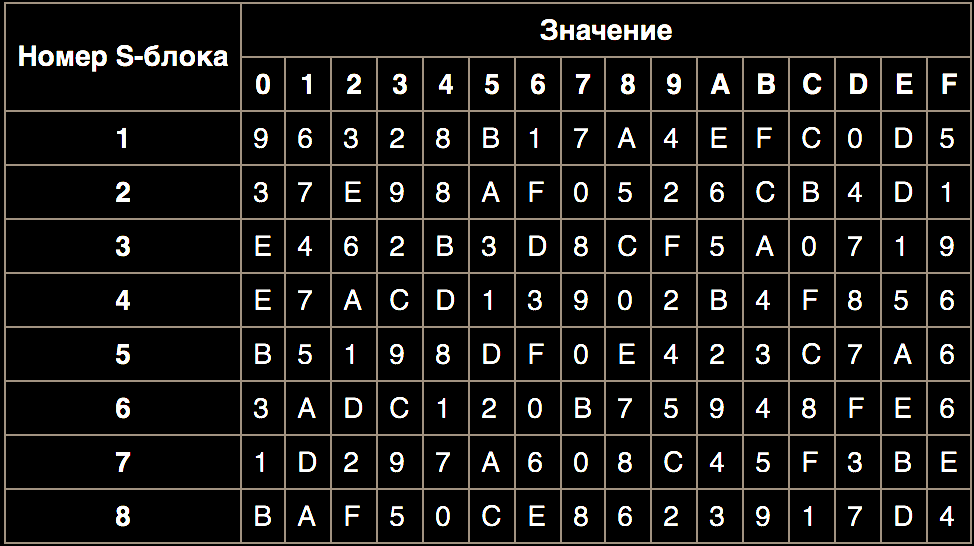
\includegraphics[width=0.77\textwidth]{Sbox_GOST}
			\hspace{5em}
	\end{figure}
\vfill
\small
{\color{gray} {Wikipedia, \url{https://ru.wikipedia.org/wiki/\%D0\%93\%D0\%9E\%D0\%A1\%D0\%A2_28147-89}}} 
\end{frame}



\begin{frame}{Подстановочно-перестановочная сеть (SPN)}
\centering
\tikzmark{start}
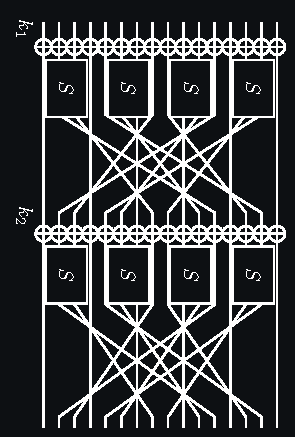
\includegraphics[height=\textheight, angle=90, origin=c]{SPN}
\tikzmark{end} 

\vfill
\small
{\color{gray} {.tex код crypto.symbols}} 

\end{frame}

\begin{frame}{AES:  SPN шифр}
\Large 
\begin{itemize}
	\itemsep 10pt
	\item стандартизирован в 2001 году (FIPS PUB 197: Advanced Encryption Standard (AES), ISO/IEC 18033-3: Block ciphers)
	\item Длина блока $n = 128 $ бит, длины ключей $k = \{128, 192, 256 \}$
	\item Количество раундов: 10 ($k = 128$), 12 ($k=192$), 14 ($k=256$)
	\item 128 бит организованы в матрицу $4 \times 4$ байт
	\[
	\begin{pmatrix}
	b_0 & b_4 & b_8 & b_{12} \\
	b_1 & b_5 & b_9 & b_{13} \\
	b_2 & b_6 & b_{10} & b_{14} \\
	b_3 & b_7 & b_{11} & b_{15}  \\
	\end{pmatrix}
	\]
\end{itemize}
%	\begin{figure}
%		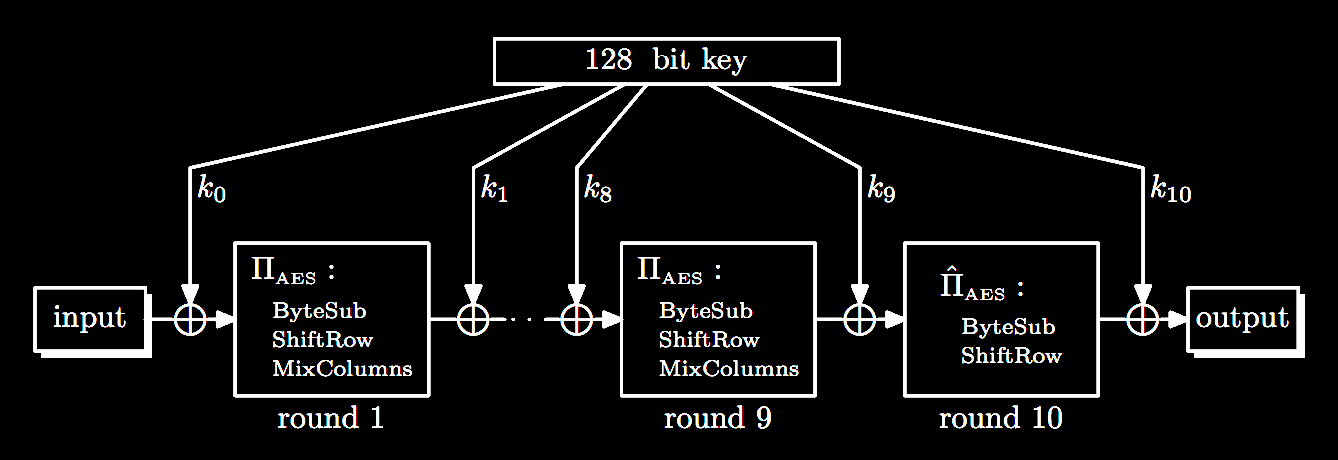
\includegraphics[width=1.1\textwidth]{AES_128}
%	\end{figure}
	
%	\Large 
%	\[
%		\Pi_{\text{AES}}  = \{0,1\}^{128} \rightarrow \{0,1\}^{128} - \text{ invertible permutation }
%	\]
%	\vfill
%	\small
%	{\color{gray}\textbf{picture is taken from D.Boneh, V.Shoup A Graduate Course in Applied Cryptography}} 
\end{frame}


\begin{frame}{Перестановка $f_{\text{AES}}$}
\Large
Перестановка $f_{\text{AES}}$ состоит из трёх обратимых операций: \\[5pt]
\begin{enumerate}
	\itemsep10pt
	\item $\mathtt{SubBytes}$ (единственная нелинейная операция)
	\[
	S: \{0,1\}^8 \rightarrow \{0,1\}^n - \text{S-бокс }
	\]
	\item  $\mathtt{ShiftRows}$
	\[
	\begin{pmatrix}
	b_0 & b_4 & b_8 & b_{12} \\
	b_1 & b_5 & b_9 & b_{13} \\
	b_2 & b_6 & b_{10} & b_{14} \\
	b_3 & b_7 & b_{11} & b_{15}  \\
	\end{pmatrix}
	\rightarrow
	\begin{pmatrix}
	b_0 & b_4 & b_8 & b_{12} \\
	b_5 & b_9 & b_{13} & b_1 \\
	b_{10} & b_{14} & b_{2} & b_{6} \\
	b_{15} & b_{3} & b_{7} & b_{11}  \\
	\end{pmatrix}
	\]
	
	\item  $\mathtt{MixColumns}$ -- столбцы перемешиваются по определённому \\ правилу (см. \url{en.wikipedia.org/wiki/Advanced_Encryption_Standard})

%	\[
%		\begin{pmatrix}
%		 \\
%		 b^{\text{new}}_j \\
%		\\
%		\end{pmatrix}
%		= 
%		\begin{pmatrix} 
%		2 & 3 & 1 & 1 \\
%		1 & 2 & 3 & 1 \\
%		1 & 1 & 2 & 3 \\
%		3 & 1 & 1 & 2 
%		\end{pmatrix}
%		\cdot
%		\begin{pmatrix}
%		\\
%		b_j \\
%		\\
%		\end{pmatrix}
%	\]
	
\end{enumerate}

\vspace{20pt}

Принцип: минимизировать успешность известных атак.	

\end{frame}

\begin{frame}{Расширение ключа в AES}
	\Large
	Задача: расширить ключ $k  \in \{0,1\}^{128}$ до 10 раундовых ключей $k_i \in \{0,1\}^{128}$
	
	\vspace{20pt}
	
	\LARGE
	\begin{itemize}
		\itemsep 10pt
		\item $k_0 = k = (w_{0,0}, w_{0,1}, w_{0,2}, w_{0,3})$, $w_{0,1} \in \{0,1\}^{32}$
		
		\item $k_i = (w_{i,0}, w_{i,1}, w_{i,2}, w_{i,3})$, где
		\begin{align*}
			w_{i,0} &= w_{i-1, 0} \oplus g_i(w_{i-1, 3}) \\	
			w_{i,1} &= w_{i-1, 1} \oplus w_{i, 0} \\
			w_{i,2} &= w_{i-1, 2} \oplus w_{i, 1} \\
			w_{i,3} &= w_{i-1, 3} \oplus w_{i, 2} \\
		\end{align*}
		$g_i : \{0,1\}^{32} \rightarrow \{0,1\}^{32}  $ -- функция, состоящая из сдвигов, \\ подстановки $\mathtt{SubBytes}$ и $\mathtt{XOR}$ с раундовыми константами $c_i$.
	\end{itemize}
\end{frame}

\begin{frame}
Часть II \\ [10pt]
\begin{LARGE}
	
	\color{Orange}
	\Huge Атаки на блочные шифры
	
\end{LARGE}
\end{frame}

\begin{frame}{Блок-шифр}
\begin{figure}
	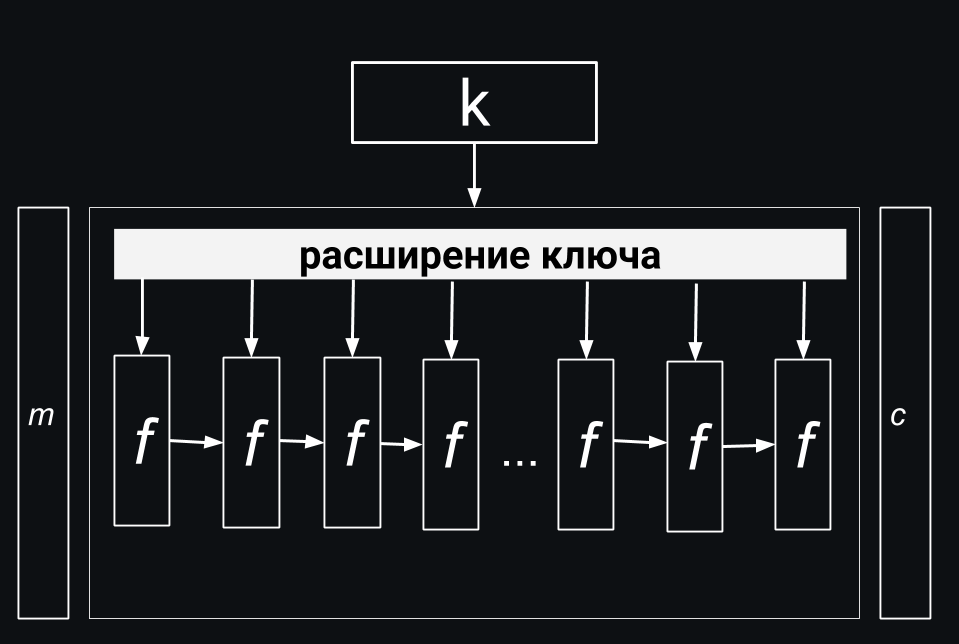
\includegraphics[width=0.7\textwidth]{BlockCipherGeneral}
\end{figure}

\end{frame}



\begin{frame}{Алгоритм перебора}

\Large
{\color{Orange}\textbf{Идея:}}  перебор ключа $k \in \{0,1\}^{\kappa}$ \\[5pt]

Для DES/AES/GOST:  достаточно двух пар (открытый текст, шифр-текст) $(m_1, c_1 = \Enc(k, m_1)), (m_2, c_2=\Enc(k,m_2))$, чтобы определить $k$ с большой вероятностью.\\[10pt]

{\color{Orange}\textbf{Сложность:}} $\bigO(2^{\kappa})$ \\[10pt]

{\color{Orange}\textbf{Пример:}}  DES $k \in \{0,1\}^{56}$:

\begin{itemize}
\item {\color{Orange}\textbf{'99-e}} ~22 часа на DeepCrack: дорогое железо+распределенная сеть
\item {\color{Orange}\textbf{'07-е}}~13 дней COPACOBANА: FPGA, дешевле
\end{itemize}
\end{frame}


\begin{frame}{Атаки на дизайн }
\LARGE
\begin{itemize}
	\itemsep 1em
	\item Линейный криптанализ:  \\[2pt]
	аппроксимация S-box линейной функцией
	
	\item дифференциальный криптоанализ \\[5pt]
\end{itemize}
\end{frame}


\begin{frame}{Атаки на реализацию}
\LARGE
\begin{itemize}
\itemsep 1em
\item Атаки по сторонним каналам (side-channel attacks): \\[2pt]
замер {\color{Orange}\textbf{времени}} или {\color{Orange}\textbf{мощности}}, используемых в процессе $\Enc, \Dec$   \\[5pt]
Эти величины не должны зависеть от секретного ключа.

\item Внесение неисправностей (Fault-injection attacks)  \\[5pt]
внешние воздействия на устройство, порождения аппаратных ошибок (нагрев, ЭМ волны)
\end{itemize}
\end{frame}


\begin{frame}{Советы}
\Huge

\begin{enumerate}
\itemsep 1em
\item {\color{Orange}\textbf{Не}} изобретайте {\color{Orange}\textbf{свой собственный}}  блок-шифр
\item {\color{Orange}\textbf{Используйте}} реализации блок-шифров из проверенных временем библиотек

\end{enumerate}
\end{frame}

\begin{frame}{Что почитать}
	\begin{figure}
		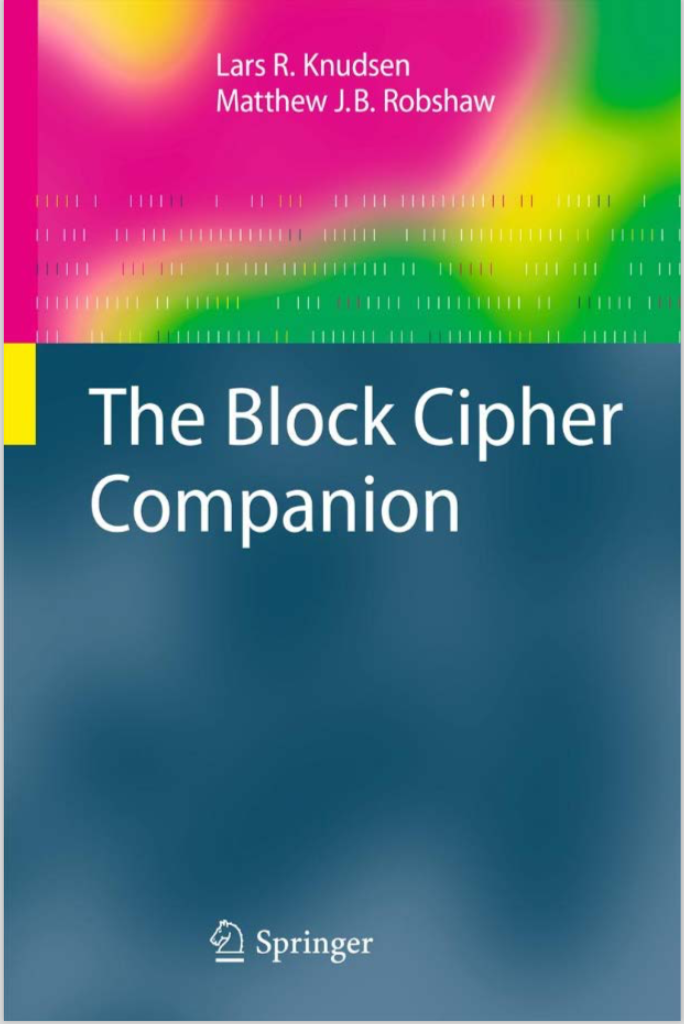
\includegraphics[height=0.7\textheight]{Book_cover}
	\end{figure}
\end{frame}

\begin{frame}
Часть III \\ [10pt]
\begin{LARGE}
	
	\color{Orange}
	\Huge Режим шифрования (modes of operation)
	
\end{LARGE}
\end{frame}

\begin{frame}
\Huge
\centering
{\color{Orange}Как правильно использовать блочный шифр для шифрования сообщений?} \\[10pt]

\end{frame}

\begin{frame}{Режимы шифрования}
\LARGE
\centering
\begin{enumerate} 
\itemsep 10pt
\item Режим электронной кодовой книги или режим простой замены (Electronic Block Code, EBC)
\item Режим сцепления блоков шифротекста (Cipher Block Chain, CBC)
\item Режим счётчика (Counter mode, CTR)
\end{enumerate}

\end{frame}

\begin{frame}{Электронная кодовая книга, Electronic Block Code (EBC)}

\Large
Пусть $m = (m_1, m_2, m_3, ...), m_i \in \{0,1\}^n$ -- открытый текст. \\[10pt]
Наивный способ  использования блочного шифра $B$
\begin{figure}
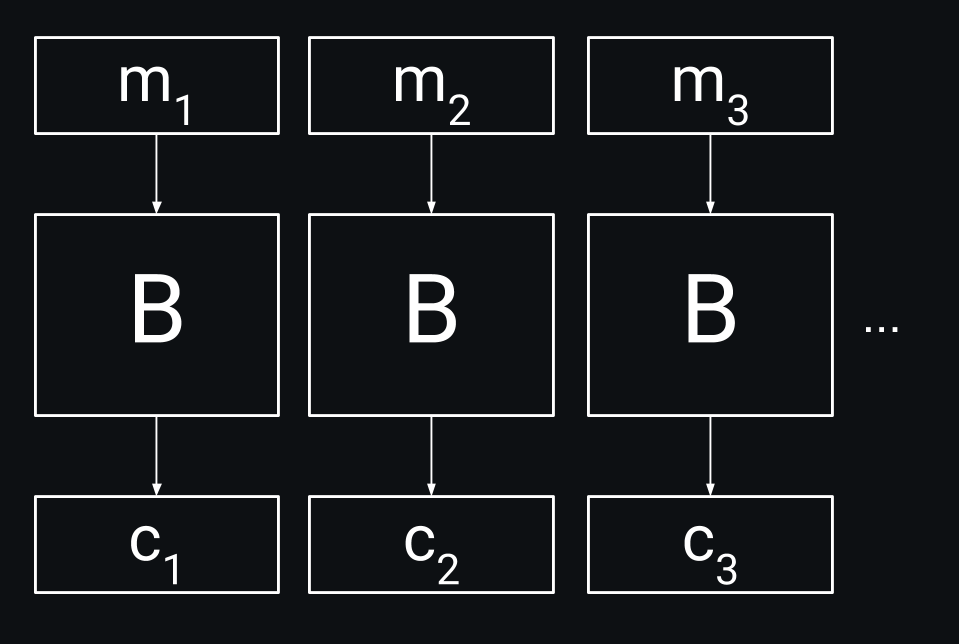
\includegraphics[width=0.65\textwidth]{EBC}
\end{figure}
\LARGE
Это {\color{Orange} небезопасный!} метод: \quad
если $m_1 = m_2$, то $c_1 = c_2$.

\end{frame}

\begin{frame}{Небезопасность EBC}
\centering
\Huge Если $m_1 = m_2$, то $c_1 = c_2$ \\[20pt]
\large
\begin{figure}
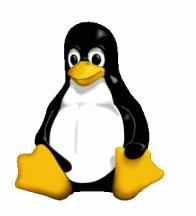
\includegraphics[width=0.22\textwidth]{Tux} \quad 
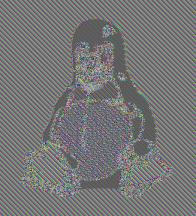
\includegraphics[width=0.22\textwidth]{Tux_ecb} \quad 

\includegraphics[width=0.22\textwidth]{Tux_secure}
\end{figure}

\vfill
\small
{\color{gray} \textsuperscript{\textcopyright} Wikipedia} 
\end{frame}

\begin{frame}{Режим сцепления блоков, Cipher Block Chain (CBC)}
\Large
{\color{Orange} IV} -- инициализирующий (начальный) вектор -- случайная строка $n$-бит

\begin{figure}
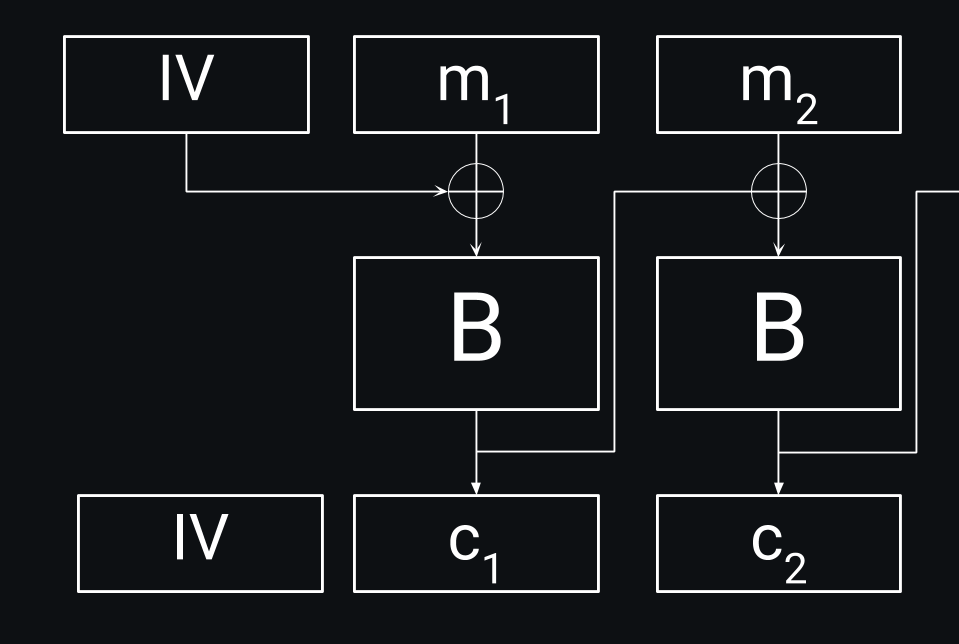
\includegraphics[width=0.7\textwidth]{CBC}
\end{figure}
IV передается с шифр-текстом (публично известно).
\end{frame}

\begin{frame}{Безопасность режима сцепления блоков}
\Large
\begin{itemize}
\itemsep 10pt
\item Начальное значение IV должно быть {\color{Orange} случайным} (если атакующий может предсказать IV, шифрование CBC небезопасно).\\ 
См. атаку на TLS 1.1.

\item{\color{Orange} IV необходимо обновлять}  \\

\end{itemize}
\end{frame}

\begin{frame}{Безопасность режима сцепления блоков}
\Large
Положим, мы используем одно и тоже IV для длинного сообщения $m=(m_1, \ldots, m_t)$ при $t> 2^{n/2}$.
\vspace{-2pt}
\begin{figure}
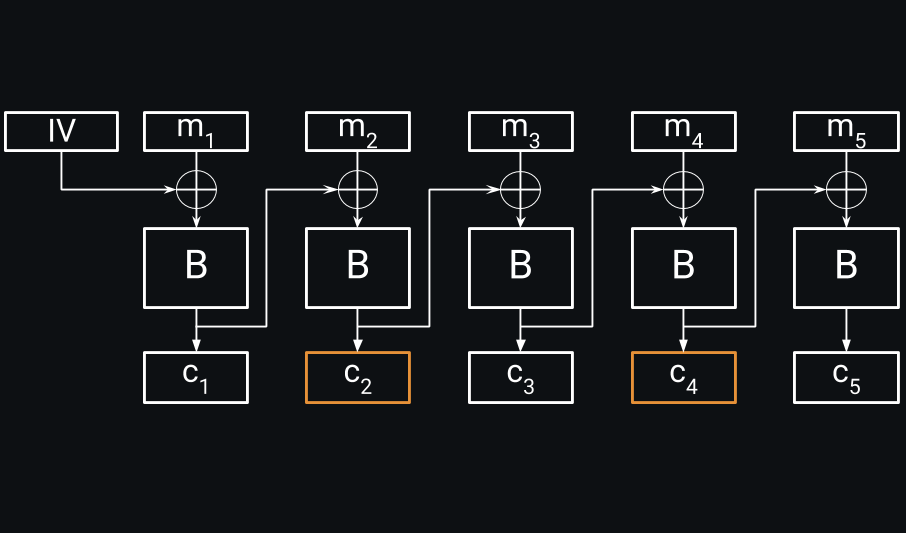
\includegraphics[width=0.7\textwidth]{CBC_1}
\end{figure}
\vspace{-35pt}
{\color{Orange}Парадокс Дней Рождений:} имея ~$2^{n/2}$ блоков шифр-текста $c_i$, \\ с большой вероятностью мы увидим два одинаковых $c_i$.
\Large
\[
c_1 \oplus m_2 == c_3 \oplus m_4
\]
Далее применяются статистические атаки на $m$.
\end{frame}

\begin{frame}{Парадокс Дней Рождений}
\Large
{\color{Orange} Определить вероятность того, что в комнате из 30 человек двое родились в один день.}\\
\pause
\vspace{30pt}
\[
\left(1 - \frac{1}{365}\right)  \left(1 - \frac{2}{365}\right) \left(1 - \frac{3}{365}\right) \cdot \ldots \cdot \left(1 - \frac{29}{365}\right)  \approx 0.294
\]

\vspace{30pt}
Значит, с вероятностью $1-0.294>0.7$ найдутся двое таких людей.

\end{frame}

\begin{frame}{Обобщение Парадокса Дней Рождений}
\Large
Для $m$ человек и $N$ возможных дней рождений, вероятность того, что все $m$ человек имеют разные дни рождения:
\[
P : = \prod_{i=1}^{m-1} \left(  1  -\frac{i}{N} \right) \approx e^{-m^2/2N}
\]

Для $m = \sqrt{2N \ln 2}$, $P \approx 1/2$.  Вероятность $P$ быстро увеличивается при росте $m$. \\[10pt]

\pause
Для блок-шифра с длиной блока $n$, имеем $2^{n}$ всевозможных блоков шифр-текстов.\\
При {\color{Orange} $m = \bigO(2^{n/2})$ } шифр-блоков $c_i$'s, некоторые два из них равны с константной вероятностью.\\[15pt]

Для режима CBC: $c_i == c_j$ при $m=(m_1, \ldots, m_t)$, {\color{Orange} $t \approx 2^{n/2}$}:
\Large
\[
{\color{Orange} c_{i-1} \oplus m_{i} == c_{j-1} \oplus m_{j}}
\]

\end{frame}


\begin{frame}{Набивка (Padding) для режима CBC}
\Large
CBC подразумевает, что все блоки $m_i$ фиксированной длины. Для этого используется ``набивка''.
\begin{figure}
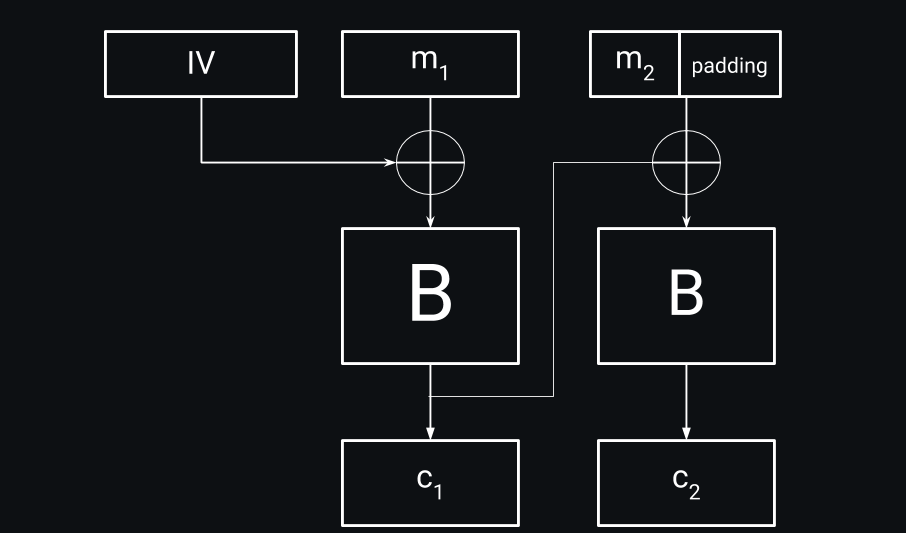
\includegraphics[width=0.70\textwidth]{CBC_Padding}
\end{figure}
Обычно $\ell$-байтная набивка состоит из $\ell$ копий of $\ell$. \\
Набивка из $5$ байт: $5|5|5|5|5$. \\
Если $m$ занимает меньше $n$-бит, добавляется фиктивный (dummy) блок.
\end{frame}

\begin{frame}{Режим счетчика, Counter Mode (CTR)}
\Large
Один из самых популярных режимов шифрования \\
Здесь IV - начальное значение счетчика. \\
Счетчик увеличивается для каждого нового блока. \\
\begin{figure}
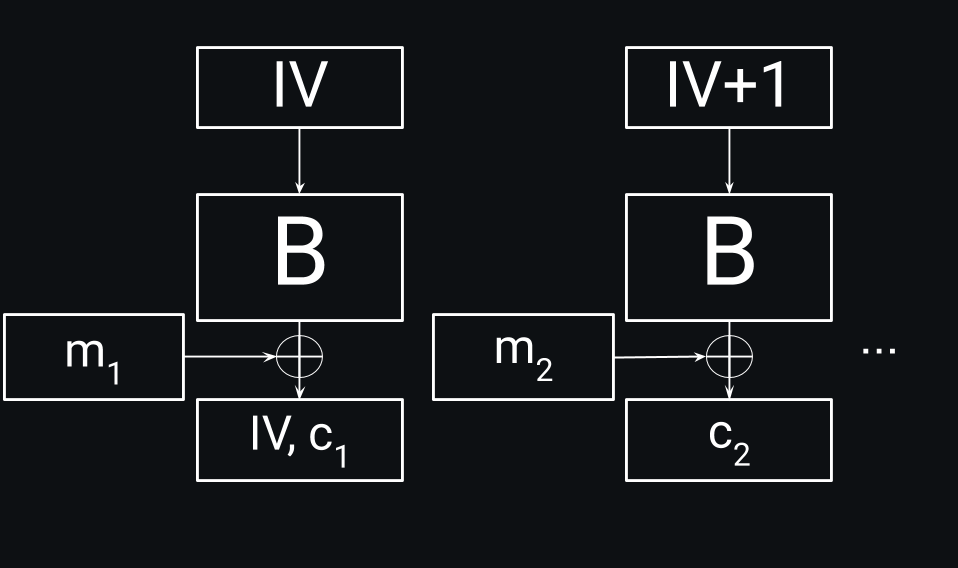
\includegraphics[width=0.75\textwidth]{CTR}
\end{figure}
\vspace{-20pt}
CTR создает потоковое шифрование из блок-шифра \\

\end{frame}

\begin{frame}{Как выглядит IV}
\begin{figure}
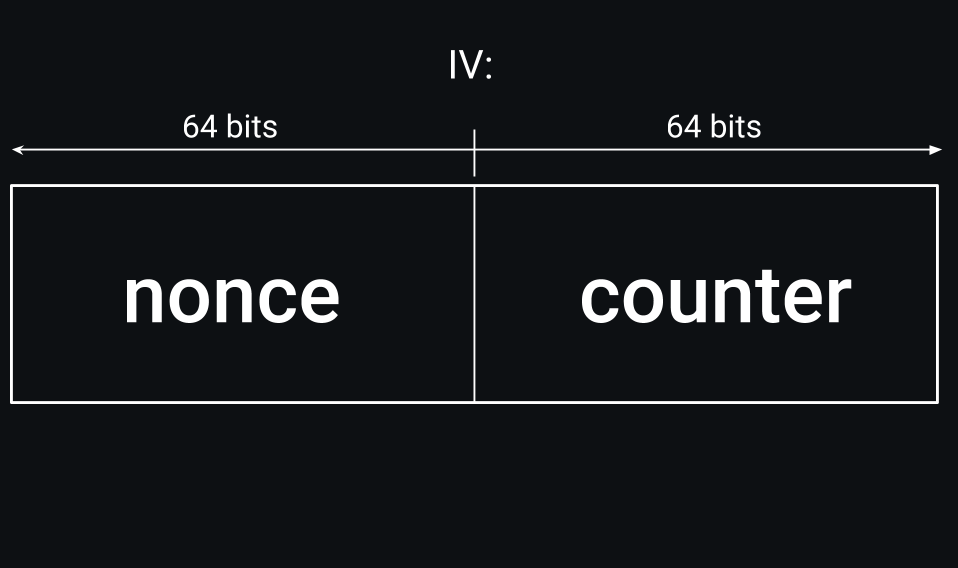
\includegraphics[width=0.70\textwidth]{ShapeOfIV}
\end{figure}
\vspace*{-50pt}
\large
\begin{itemize}
\item Nonce (нонс) должен быть псевдослучайным (64-битный выход PRG) и \\ не должен повторяться для одного и того же ключа $k$\\
\item Счетчик увеличивается для каждого нового блока
\item Значение счетчика не передается в протоколах, обеспечивающих \\ последовательную доставку пакетов (https)
\item Нонс обновляется после $2^{64}$ зашифрованных блоков.

\end{itemize}
\end{frame}


\begin{frame}{Преимущества режима Counter Mode}
%\vspace{-40pt}
\begin{figure}
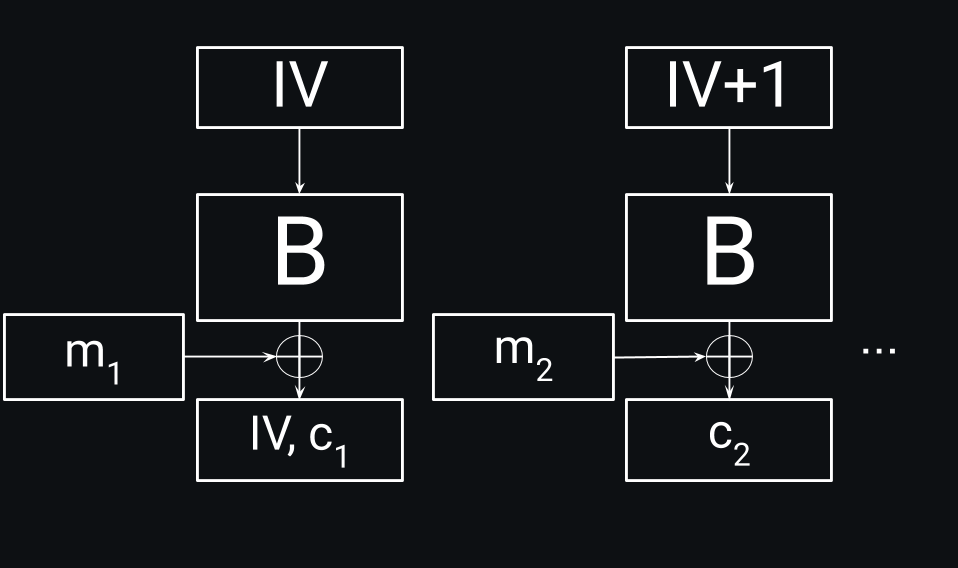
\includegraphics[width=0.55\textwidth]{CTR}
%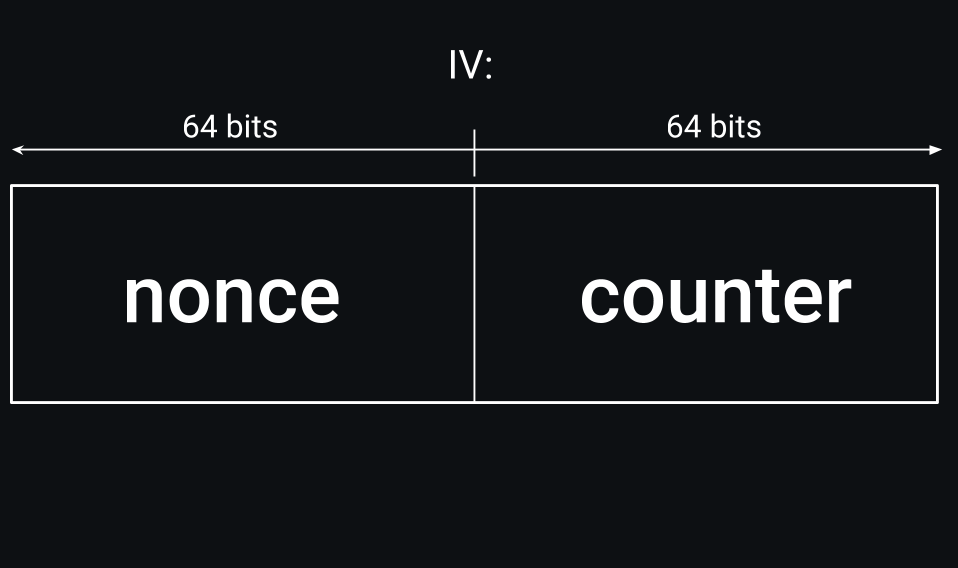
\includegraphics[width=0.5\textwidth]{ShapeOfIV}
\end{figure}
\vspace{-20pt}
\Large
\begin{itemize}
\item Нонс известен шифрующей и дешифрующей сторонам
\item Простая процедура дешифрования
\item Лёгкая параллелизация (в отличие от CBC)
\item Не нужно использовать набивку
\item 64-битный нонс (CTR) vs.\ 128-битный IV
\end{itemize}

\end{frame}



\end{document}